\documentclass{article}%
\usepackage[T1]{fontenc}%
\usepackage[utf8]{inputenc}%
\usepackage{lmodern}%
\usepackage{textcomp}%
\usepackage{lastpage}%
\usepackage[head=40pt,margin=0.5in,bottom=0.6in]{geometry}%
\usepackage{graphicx}%
%
\title{\textbf{Familiares exigen libertad plena para presos políticos antes de Navidad}}%
\author{RAFAEL LEÓN | Raleon@el{-}nacional.com}%
\date{04/12/2018}%
%
\begin{document}%
\normalsize%
\maketitle%
\textbf{URL: }%
http://www.el{-}nacional.com/noticias/politica/familiares{-}exigen{-}libertad{-}plena{-}para{-}presos{-}politicos{-}antes{-}navidad\_262037\newline%
%
\textbf{Periodico: }%
EN, %
ID: %
262037, %
Seccion: %
Política\newline%
%
\textbf{Palabras Claves: }%
NO\_TIENE\newline%
%
\textbf{Derecho: }%
1.2, %
Otros Derechos: %
, %
Sub Derechos: %
1.2.2\newline%
%
\textbf{EP: }%
NO\newline%
\newline%
%
\textbf{\textit{Este año 300 detenidos, de acuerdo con la Coalición por los Derechos Humanos y la Democracia, pasarán por primera vez la Navidad fuera de su hogar. Parientes esperan que el gobierno dé muestra de reconciliación a través de su liberación de los encarcelados por razones políticas}}%
\newline%
\newline%
%
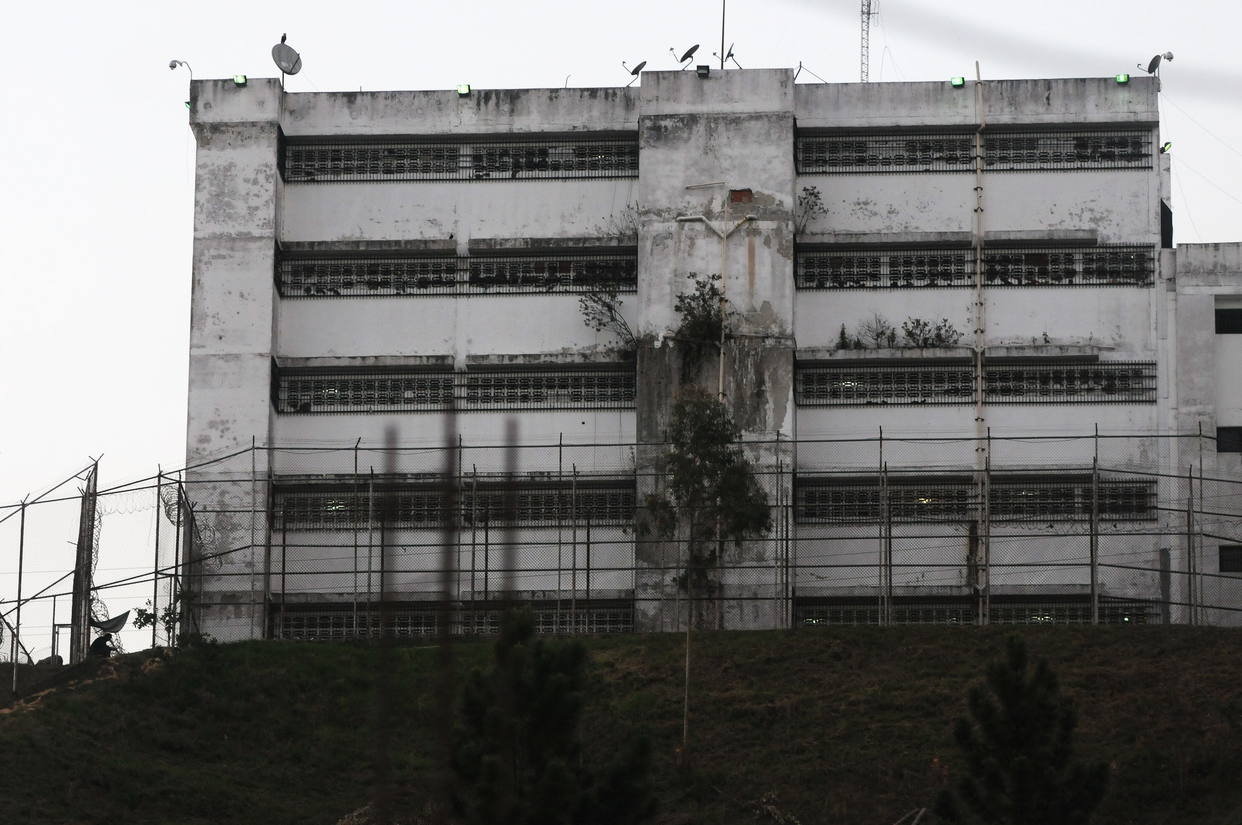
\includegraphics[width=300px]{215.jpg}%
\newline%
%
Un total de 14 nochebuenas consecutivas tiene separada a la familia Guevara{-}Sandoval. Desde 2003 Jackeline Sandoval no celebra el 24 de diciembre junto a su esposo, Rolando Guevara, quien desde hace 14 años se encuentra preso por razones políticas y, a pesar de haber cumplido un cuarto de la pena, han ignorado las solicitudes de medidas alternativas de privación de libertad.%
\newline%
%
“Como en Navidad y en cualquier época del año esperamos la liberación de nuestros familiares. Llevamos 14 años sin tener unas navidades completas. No podemos pasarla bien; por más que uno trate de hacer una cena, nunca vamos a disfrutarla si uno de los miembros de la familia está encarcelado”, expresó Sandoval. Ella, al igual que otros familiares y abogados, exigió al gobierno la libertad para todos los presos políticos que, de acuerdo con el Foro Penal Venezolano, suman 288 personas mientras que la Coalición por los Derechos Humanos y la Democracia registra 402 encarcelados.%
\newline%
%
Abogan por que al igual que el año pasado el gobierno ejecute mecanismos para otorgar excarcelar a sus parientes. Tal es el caso de Ana María da Costa, hermana de Vasco da Costa, quien se encuentra preso en la cárcel de Santa Ana por estar presuntamente involucrado en la Operación Gedeón II.%
\newline%
%
“Nuestra exigencia es la libertad plena de todos los presos políticos antes de Navidad. Para estas fechas es triste porque tenemos a Vasco preso, porque la está pasando mal, porque está sufriendo y nosotros también”, manifestó.%
\newline%
%
Son cientos de hogares en los que este 24 de diciembre sobrará una silla durante la cena navideña. De acuerdo con Ana Leonor Acosta, abogado de la Coalición por los Derechos Humanos y la Democracia, son alrededor de 300 encarcelados políticos los que se han registrado este año, muchos de los cuales se encuentran enfermos.~Pidió que “se eliminen las medidas cautelares a las que están sujetos miles de personas”.%
\newline%
%
Este sería el primer año para Sabina y Mariano sin tener a su padre en casa, el diputado Juan Requesens, por lo cual su esposa, Oriana Granatti, exigió al gobierno que cumpla con el Estado de Derecho, y respete los derechos humanos y el debido proceso de todos los presos políticos, especialmente el del parlamentario que, según su defensa, ha sido víctima de violaciones de este último.%
\newline%
%
“Para Navidad exigimos que Juan esté libre, que se le permita estar donde debe estar con su familia. Igualmente para todos los presos políticos que están allí solo porque al régimen le molesta que la gente alce la voz”, añadió Granatti.%
\newline%
%
Alfredo Romero, director Ejecutivo del Foro Penal Venezolano, destacó que esta fecha es una oportunidad para que el gobierno disminuya su costo moral ante la comunidad internacional por las denuncias que tiene en su contra por violaciones a los derechos humanos.%
\newline%
%
El abogado manifestó que este año se ha caracterizado por la persecución al sector militar, las detenciones de familiares de los objetivos políticos y por la utilización de la tortura. Este último mecanismo, que ha dejado secuelas graves para las víctimas, entre ellas los médicos William Aguado, quien tiene un problema renal y no ha recibido atención médica; José Marulanda, quien sufrió fracturas en las manos, y el general José Gámez, quien se encuentra en la cárcel 26 de Julio, en Guárico, en estado de desnutrición y ha sufrido un ACV en dos oportunidades debido a la situación de reclusión.%
\newline%
%
“Mis navidades son muy tristes. Después de cuatro años en prisión es la primera vez que estaré libre y es horrible pensar en las condiciones en las que estará mi esposo”, expresó Carmen Gutiérrez, ex presa política y esposa de Gámez.%
\newline%
%
Denuncian golpiza en Ramo Verde%
\newline%
%
Familiares de Yofran Quintero, a quien acusan de estar involucrado en la Operación Gedeón II, denunciaron que el joven recibió una fuerte golpiza de parte de funcionarios de la cárcel militar de Ramo Verde, donde se encuentra detenido.%
\newline%
%
A través de un comunicado, los parientes exigieron que Quintero sea chequeado por un médico forense para que certifique su estado físico. Responsabilizaron al presidente Nicolás Maduro; al ministro de Interior y Justicia, Nestor Reverol; al ministro de la Defensa, Vladimir Padrino, y al juez Maikel Amezquita Pionner por la vida y la integridad del joven quien, al igual que los otros seis involucrados en el caso, se define como dirigente nacionalista.%
\newline%
%
EL DATO%
\newline%
%
Joel García, abogado del diputado Juan Requesens, anunció que luego de 111 días de retraso el tribunal fijó la audiencia preliminar para el 18 de diciembre. Informó que la comparecencia será a las 10:30 am y el presidente Nicolás Maduro debe acudir. Indicó que tuvieron acceso al expediente y “no hay elementos para afirmar que Requesens es partícipe de los hechos que se le imputan”.%
\newline%
%
\end{document}